\documentclass[12pt]{article}

% Idioma e codificação
\usepackage[brazil]{babel}
\usepackage[utf8]{inputenc}
\usepackage[T1]{fontenc}

% Matemática e listas
\usepackage{amsmath, amssymb}
\usepackage{enumitem}

% Layout e cores
\usepackage{geometry}
\usepackage{graphicx}
\usepackage{xcolor}

% Diagramas e Portas Lógicas
\usepackage{tikz}
\usetikzlibrary{shapes.gates.logic.US, positioning, arrows.meta, calc, fit, shadows.blur, shapes.geometric}
\usepackage{listings}

% --- Estilo listings: Kotlin ---
\definecolor{kotlinpurple}{RGB}{122, 44, 191}
\definecolor{codeblue}{RGB}{0, 79, 151}
\definecolor{codegray}{RGB}{128, 128, 128}
\definecolor{codegreen}{RGB}{30, 130, 60}
\definecolor{codebg}{RGB}{245, 245, 250}

\lstdefinelanguage{Kotlin}{
  keywords={fun, val, var, if, else, for, while, return, import, class, object, null, true, false, in, is, as, when, by, companion, override, data, sealed, interface, abstract, open, private, public, internal, protected, suspend, coroutine, out, in},
  keywordstyle=\bfseries\color{kotlinpurple},
  ndkeywords={String, Int, Boolean, Double, Float, Long, Array, List, ArrayList, Unit},
  ndkeywordstyle=\color{codeblue},
  sensitive=true,
  comment=[l]{//},
  morecomment=[s]{/*}{*/},
  commentstyle=\itshape\color{codegray},
  stringstyle=\color{codegreen},
  morestring=[b]",
}

\lstdefinestyle{KotlinStyle}{
  language=Kotlin,
  basicstyle=\ttfamily\small,
  backgroundcolor=\color{codebg},
  frame=single,
  rulecolor=\color{kotlinpurple},
  numbers=none,
  breaklines=true,
  showstringspaces=false,
  tabsize=2,
  literate=
    {á}{{\'{a}}}1 {à}{{\`{a}}}1 {ã}{{\~{a}}}1 {â}{{\^{a}}}1
    {é}{{\'{e}}}1 {ê}{{\^{e}}}1
    {í}{{\'{i}}}1
    {ó}{{\'{o}}}1 {õ}{{\~{o}}}1 {ô}{{\^{o}}}1
    {ú}{{\'{u}}}1
    {ç}{{\c{c}}}1
    {Á}{{\'{A}}}1 {É}{{\'{E}}}1 {Í}{{\'{I}}}1 {Ó}{{\'{O}}}1 {Ú}{{\'{U}}}1
    {Ç}{{\c{C}}}1,
}

% Cores institucionais
\definecolor{maincolor}{RGB}{0, 79, 151}
\definecolor{meuazul}{RGB}{0, 79, 151}

% Cabeçalho e rodapé
\usepackage{fancyhdr}

% Blocos
\usepackage[most]{tcolorbox}
\newtcolorbox{block}[1]{%
  colback=blue!5,
  colframe=maincolor,
  coltitle=white,
  title=#1,
  fonttitle=\bfseries,
  boxrule=1.5pt,
  arc=3mm,
  left=6pt,
  right=6pt,
  top=6pt,
  bottom=6pt
}

\newtcolorbox{resposta}[1]{%
  colback=white,
  colframe=meuazul!30,
  arc=1mm,
  height=#1,
  width=\textwidth,
  boxrule=0.8pt
}

% Margens
\geometry{margin=2.5cm}

% Fancyhdr
\pagestyle{fancy}
\fancyhf{}

\renewcommand{\headrulewidth}{2pt}
\renewcommand{\footrulewidth}{2pt}

\renewcommand{\headrule}{\hbox to\headwidth{%
  \color{meuazul}\leaders\hrule height \headrulewidth\hfill}}

\renewcommand{\footrule}{\hbox to\headwidth{%
  \color{meuazul}\leaders\hrule height \footrulewidth\hfill}}

\setlength{\headheight}{52pt}
\addtolength{\topmargin}{-20pt}

\fancyhead[L]{%
  
\includegraphics[height=1.2cm]{./../logo.png}
}

\fancyhead[R]{%
  \raggedleft
  \textcolor{meuazul}{%
    \small
    \textbf{Lista de Exercícios — Desenvolvimento de Software para Dispositivos Móveis}\\
    Me.~Sergio Souza Novak\\
    \textit{Engenharia da Qualidade e Confiabilidade}
  }
}

\fancyfoot[C]{\textcolor{meuazul}{\thepage}}

% =========================
\begin{document}

\vspace*{0.2cm}

\begin{center}
  {\Large \textbf{Lista de Exercícios — Introdução à Linguagem Kotlin e POO}}\\[0.2cm]
  \textit{\textbf{Instruções de Entrega:} Os alunos devem desenvolver o código-fonte em Kotlin para cada um dos problemas. A solução final deve ser compactada e submetida no \textbf{Google Classroom} em um arquivo \textbf{.zip} contendo os arquivos ou pastas organizados como \texttt{exercicio1}, \texttt{exercicio2}, \texttt{exercicio3}, \texttt{exercicio4}, \texttt{exercicio5} e \texttt{exercicio6}.}
\end{center}

\vspace{0.4cm}

\begin{center}
  \textit{``Boa atividade! Att. Me. Prof. Sergio Souza Novak.''}
\end{center}

\vspace{0.4cm}

% =========================================================================
% Questão 1 — Média Aritmética
% =========================================================================
\noindent\textbf{Questão 1 — Cálculo de Média Aritmética e Situação Acadêmica (\texttt{exercicio1})}

\vspace{0.2cm}
\noindent
Escreva um programa em Kotlin que receba três notas de um aluno (valores do tipo \texttt{Double}), calcule a média aritmética simples e determine a situação acadêmica do estudante segundo os seguintes critérios:
\begin{itemize}[leftmargin=1.5em]
  \item Média $\ge 7.0$: "Aprovado"
  \item $5.0 \le$ Média $< 7.0$: "Em Recuperação"
  \item Média $< 5.0$: "Reprovado"
\end{itemize}
\textbf{Requisito:} Implemente uma função `calcularMedia(n1: Double, n2: Double, n3: Double): Double` e utilize \textit{string templates} para formatar a saída com duas casas decimais.

\vspace{0.2cm}
\begin{block}{Exemplo de Entrada e Saída Esperada (Console)}
\textbf{Entrada no código / teclado:} \texttt{Nota 1 = 8.5}, \texttt{Nota 2 = 6.0}, \texttt{Nota 3 = 7.5}\\
\textbf{Saída de Console:}
\begin{verbatim}
Notas digitadas: 8.5, 6.0, 7.5
Média do aluno: 7.33
Situação: Aprovado
\end{verbatim}
\end{block}

\vspace{0.6cm}
\noindent\rule{\textwidth}{0.8pt}
\vspace{0.4cm}

% =========================================================================
% Questão 2 — Manipulação de Strings
% =========================================================================
\noindent\textbf{Questão 2 — Analisador e Formatador de Nomes de Usuários (\texttt{exercicio2})}

\vspace{0.2cm}
\noindent
Em aplicativos móveis, a higienização e validação de strings digitadas pelo usuário são essenciais. Crie um programa em Kotlin que receba um nome completo digitado (exemplo: \texttt{"  sergio souza novak  "}) e realize as seguintes operações de manipulação de String:
\begin{enumerate}[label=\alph*), leftmargin=1.5em]
  \item Remova espaços desnecessários no início e no fim da string.
  \item Converta o nome para letras maiúsculas.
  \item Conte a quantidade de vogais (a, e, i, o, u) presentes no nome.
  \item Verifique se o nome contém o sobrenome \texttt{"Novak"} (ignorando diferenças entre maiúsculas e minúsculas).
  \item Gere um nome de exibição no formato: \texttt{"PrimeiroNome SOBRENOME"} (exemplo: \texttt{"Sergio NOVAK"}).
\end{enumerate}

\vspace{0.2cm}
\begin{block}{Exemplo de Entrada e Saída Esperada (Console)}
\textbf{Entrada:} \texttt{"  sergio souza novak  "}\\
\textbf{Saída de Console:}
\begin{verbatim}
Nome higienizado: "sergio souza novak"
Nome em maiúsculas: SERGIO SOUZA NOVAK
Quantidade de vogais: 8
Contém sobrenome 'Novak'? sim
Nome de Exibição: Sergio NOVAK
\end{verbatim}
\end{block}

\vspace{0.6cm}
\noindent\rule{\textwidth}{0.8pt}
\vspace{0.4cm}

% =========================================================================
% Questão 3 — Busca Binária
% =========================================================================
\noindent\textbf{Questão 3 — Busca Binária em Coleção de Dados Ordenada (\texttt{exercicio3})}

\vspace{0.2cm}
\noindent
A busca binária é um algoritmo eficiente de busca com complexidade $O(\log n)$, que exige que a lista esteja previamente ordenada. 

\vspace{0.2cm}
\noindent
Implemente em Kotlin uma função `buscaBinaria(array: IntArray, chave: Int): Int` que retorna o índice onde a `chave` foi encontrada ou `-1` caso o valor não pertença ao array.
\begin{itemize}[leftmargin=1.5em]
  \item Crie uma lista/array de inteiros contendo pelo menos 10 elementos ordenados.
  \item Demonstre o teste da sua função buscando por um elemento existente e por um elemento inexistente.
  \item Imprima no console cada passo do algoritmo (valores de \texttt{inicio}, \texttt{fim} e \texttt{meio}).
\end{itemize}

\vspace{0.2cm}
\begin{block}{Exemplo de Entrada e Saída Esperada (Console)}
\textbf{Array de Entrada:} \texttt{[5, 12, 18, 23, 34, 45, 56, 67, 78, 89]}\\
\textbf{Teste 1 — Buscar chave = 56:}\\
\texttt{Passo 1: inicio=0, fim=9, meio=4 (valor 34) -> buscar à direita}\\
\texttt{Passo 2: inicio=5, fim=9, meio=7 (valor 67) -> buscar à esquerda}\\
\texttt{Passo 3: inicio=5, fim=6, meio=5 (valor 45) -> buscar à direita}\\
\texttt{Passo 4: inicio=6, fim=6, meio=6 (valor 56) -> ENCONTRADO!}\\
\textbf{Saída:} \texttt{Chave 56 encontrada no índice 6.}\\
\textbf{Teste 2 — Buscar chave = 99:}\\
\textbf{Saída:} \texttt{Chave 99 não encontrada no array (retorno -1).}
\end{block}

\vspace{0.6cm}
\noindent\rule{\textwidth}{0.8pt}
\vspace{0.4cm}

% =========================================================================
% Questão 4 — Rotação em Matriz de Pontos 2D
% =========================================================================
\noindent\textbf{Questão 4 — Operação de Rotação em Matrizes de Pontos 2D (\texttt{exercicio4})}

\vspace{0.2cm}
\noindent
No desenvolvimento de jogos e interfaces gráficas móveis, a rotação de coordenadas no plano cartesiano é uma operação vetorial e matricial fundamental. Dado um ponto $(x, y)$, a rotação por um ângulo $\theta$ (em radianos) no sentido anti-horário em relação à origem $(0,0)$ é dada pela multiplicação matricial:
\[
\begin{bmatrix} x' \\ y' \end{bmatrix} = \begin{bmatrix} \cos\theta & -\sin\theta \\ \sin\theta & \cos\theta \end{bmatrix} \begin{bmatrix} x \\ y \end{bmatrix}
\]
que resulta nas equações: $x' = x\cos\theta - y\sin\theta$ e $y' = x\sin\theta + y\cos\theta$.

\vspace{0.2cm}
\noindent
\textbf{Tarefas:}
\begin{enumerate}[label=\alph*), leftmargin=1.5em]
  \item Crie uma classe em Kotlin chamada `Ponto2D` com os atributos `x: Double` e `y: Double`.
  \item Adicione um método `rotacionar(anguloGraus: Double): Ponto2D` que retorne um \textbf{novo} `Ponto2D` com as coordenadas rotacionadas. Utilize a classe `kotlin.math` (\texttt{cos}, \texttt{sin}, \texttt{toRadians}).
  \item Desenvolva uma função que receba uma \textbf{matriz/array de pontos} (ex: os vértices de um triângulo ou polígono) e aplique a rotação em todos os pontos da matriz.
\end{enumerate}

\vspace{0.3cm}
% Diagramas em TikZ: Plano Cartesiano com a Letra 'E' Original e Rotacionada (ex: 90 graus)
\begin{center}
\begin{tikzpicture}[scale=0.68, font=\sffamily\tiny]

  % --- Figura 1: Polígono 'E' Original (Ângulo 0°) ---
  \begin{scope}[shift={(0,0)}]
    % Eixos cartesianos
    \draw[-{Stealth[length=4pt]}, line width=0.8pt, color=gray!80] (-1.2, 0) -- (4.2, 0) node[right] {$x$};
    \draw[-{Stealth[length=4pt]}, line width=0.8pt, color=gray!80] (0, -1.2) -- (0, 4.6) node[above] {$y$};
    \draw[color=gray!25, step=1cm] (-1,-1) grid (4,4);
    
    % Marcação da origem
    \node[below left, font=\tiny\bfseries] at (0,0) {$(0,0)$};
    
    % Polígono no formato da letra E
    % Coordenadas: (0,0) -> (3,0) -> (3,1) -> (1,1) -> (1,1.5) -> (2.5,1.5) -> (2.5,2.5) -> (1,2.5) -> (1,3) -> (3,3) -> (3,4) -> (0,4) -> cycle
    \filldraw[draw=maincolor, fill=blue!15, line width=1.2pt]
      (0,0) -- (3,0) -- (3,0.8) -- (1,0.8) -- (1,1.6) -- (2.5,1.6) -- (2.5,2.4) -- (1,2.4) -- (1,3.2) -- (3,3.2) -- (3,4) -- (0,4) -- cycle;
      
    % Destaque de alguns pontos/vértices do 'E'
    \fill[red!80!black] (0,4) circle (2.5pt) node[above left, color=red!80!black] {$P_1(0,4)$};
    \fill[red!80!black] (3,4) circle (2.5pt) node[above right, color=red!80!black] {$P_2(3,4)$};
    \fill[red!80!black] (3,0) circle (2.5pt) node[below right, color=red!80!black] {$P_3(3,0)$};
    
    \node[font=\small\bfseries, color=maincolor] at (1.5, -2.0) {a) Polígono 'E' Original ($\theta = 0^\circ$)};
  \end{scope}

  % Seta de Transformação / Rotação
  \draw[-{Stealth[length=6pt]}, line width=1.5pt, color=kotlinpurple] 
    (4.8, 1.8) -- (6.8, 1.8) node[midway, above, font=\small\bfseries, color=kotlinpurple] {Rotação $\theta = 90^\circ$};

  % --- Figura 2: Polígono 'E' Rotacionado em 90° ---
  % Matriz de Rotação 90°: [0 -1; 1 0] -> (x', y') = (-y, x)
  \begin{scope}[shift={(12.5,0)}]
    % Eixos cartesianos
    \draw[-{Stealth[length=4pt]}, line width=0.8pt, color=gray!80] (-4.5, 0) -- (1.5, 0) node[right] {$x'$};
    \draw[-{Stealth[length=4pt]}, line width=0.8pt, color=gray!80] (0, -1.2) -- (0, 4.2) node[above] {$y'$};
    \draw[color=gray!25, step=1cm] (-4,-1) grid (1,4);
    
    \node[below right, font=\tiny\bfseries] at (0,0) {$(0,0)$};
    
    % Polígono 'E' rotacionado 90°: cada (x,y) vira (-y, x)
    \filldraw[draw=kotlinpurple, fill=kotlinpurple!15, line width=1.2pt]
      (0,0) -- (0,3) -- (-0.8,3) -- (-0.8,1) -- (-1.6,1) -- (-1.6,2.5) -- (-2.4,2.5) -- (-2.4,1) -- (-3.2,1) -- (-3.2,3) -- (-4,3) -- (-4,0) -- cycle;
      
    % Destaque dos vértices correspondentes após a rotação 90°
    \fill[red!80!black] (-4,0) circle (2.5pt) node[below left, color=red!80!black] {$P_1'(-4,0)$};
    \fill[red!80!black] (-4,3) circle (2.5pt) node[above left, color=red!80!black] {$P_2'(-4,3)$};
    \fill[red!80!black] (0,3) circle (2.5pt) node[above right, color=red!80!black] {$P_3'(0,3)$};
    
    \node[font=\small\bfseries, color=kotlinpurple] at (-0.5, -2.0) {b) Polígono 'E' Rotacionado ($\theta = 90^\circ$)};
  \end{scope}

\end{tikzpicture}
\end{center}

\vspace{0.2cm}
\noindent
\textbf{Multiplicação Matricial para Rotação ($\theta = 90^\circ$):}
\[
\begin{bmatrix} x' \\ y' \end{bmatrix} = 
\begin{bmatrix} \cos(90^\circ) & -\sin(90^\circ) \\ \sin(90^\circ) & \cos(90^\circ) \end{bmatrix} \begin{bmatrix} x \\ y \end{bmatrix} = 
\begin{bmatrix} 0 & -1 \\ 1 & 0 \end{bmatrix} \begin{bmatrix} x \\ y \end{bmatrix} = 
\begin{bmatrix} -y \\ x \end{bmatrix}
\]
\noindent
Exemplo de multiplicação das coordenadas dos pontos vértices da matriz do polígono:
\[
P_1 = \begin{bmatrix} 0 & -1 \\ 1 & 0 \end{bmatrix} \begin{bmatrix} 0 \\ 4 \end{bmatrix} = \begin{bmatrix} -4 \\ 0 \end{bmatrix}, \quad
P_2 = \begin{bmatrix} 0 & -1 \\ 1 & 0 \end{bmatrix} \begin{bmatrix} 3 \\ 4 \end{bmatrix} = \begin{bmatrix} -4 \\ 3 \end{bmatrix}, \quad
P_3 = \begin{bmatrix} 0 & -1 \\ 1 & 0 \end{bmatrix} \begin{bmatrix} 3 \\ 0 \end{bmatrix} = \begin{bmatrix} 0 \\ 3 \end{bmatrix}
\]

\vspace{0.2cm}
% Diagrama UML TikZ para Ponto2D
\begin{center}
\begin{tikzpicture}[
  font=\sffamily\small,
  node distance=0.5cm,
  umlclass/.style={draw=maincolor, fill=blue!5, line width=1pt, rounded corners=2pt, inner sep=6pt, text width=7.5cm}
]
\node[umlclass] (ponto) {
  \centering \textbf{Ponto2D}\\[2pt]
  \hrulefill\\
  + x: Double\\
  + y: Double\\
  \hrulefill\\
  + rotacionar(anguloGraus: Double): Ponto2D\\
  + toString(): String
};
\end{tikzpicture}
\end{center}

\vspace{0.2cm}
\begin{block}{Exemplo de Entrada e Saída Esperada (Console)}
\textbf{Pontos de Entrada (Matriz/Array):} \texttt{[Ponto2D(0.0, 4.0), Ponto2D(3.0, 4.0), Ponto2D(3.0, 0.0)]}\\
\textbf{Ângulo de Rotação:} \texttt{90.0°}\\
\textbf{Saída de Console:}
\begin{verbatim}
--- Pontos Originais ---
P1: (0.00, 4.00)
P2: (3.00, 4.00)
P3: (3.00, 0.00)

--- Pontos Após Rotação de 90.0° ---
P1': (-4.00, 0.00)
P2': (-4.00, 3.00)
P3': (0.00, 3.00)
\end{verbatim}
\end{block}

\vspace{0.6cm}
\noindent\rule{\textwidth}{0.8pt}
\vspace{0.4cm}

% =========================================================================
% Questão 5 — Sistema de Conta Bancária (POO)
% =========================================================================
\noindent\textbf{Questão 5 — Sistema de Conta Bancária com Operações Financeiras (\texttt{exercicio5})}

\vspace{0.2cm}
\noindent
Modele e implemente em Kotlin um sistema de conta bancária orientada a objetos com base no diagrama de classe UML a seguir:

\vspace{0.2cm}
% Diagrama UML TikZ para ContaBancaria
\begin{center}
\begin{tikzpicture}[
  font=\sffamily\small,
  umlclass/.style={draw=maincolor, fill=blue!5, line width=1pt, rounded corners=2pt, inner sep=6pt, text width=9.5cm}
]
\node[umlclass] (conta) {
  \centering \textbf{ContaBancaria}\\[2pt]
  \hrulefill\\
  + numeroConta: String\\
  + titular: String\\
  - saldo: Double\\
  \hrulefill\\
  + constructor(numeroConta: String, titular: String, saldoInicial: Double)\\
  + depositar(valor: Double): Boolean\\
  + sacar(valor: Double): Boolean\\
  + transferir(destino: ContaBancaria, valor: Double): Boolean\\
  + consultarSaldo(): Double
};
\end{tikzpicture}
\end{center}

\vspace{0.2cm}
\noindent
\textbf{Regras de Negócio:}
\begin{itemize}[leftmargin=1.5em]
  \item O atributo \texttt{saldo} deve ser estritamente privado (\texttt{private}).
  \item O método `depositar(valor)` só deve aceitar valores estritamente positivos ($>0$).
  \item O método `sacar(valor)` deve verificar se há saldo suficiente para realizar a operação.
  \item O método `transferir(destino, valor)` deve debitar da conta de origem e creditar na conta de `destino` apenas se o saque de origem for bem-sucedido.
  \item No `main()`, crie duas contas, realize depósitos, saques e uma transferência entre elas, exibindo os saldos finais.
\end{itemize}

\vspace{0.2cm}
\begin{block}{Exemplo de Entrada e Saída Esperada (Console)}
\textbf{Operações no \texttt{main()}:} 
Criar \texttt{c1("101-X", "Sergio", 1000.0)} e \texttt{c2("202-Y", "Ana", 500.0)}.\\
Depositar R\$ 200 em c1 | Sacar R\$ 150 de c2 | Transferir R\$ 300 de c1 para c2.\\
\textbf{Saída de Console:}
\begin{verbatim}
[Depósito] R$ 200.0 depositado na conta 101-X (Sergio). Saldo: R$ 1200.0
[Saque] R$ 150.0 sacado da conta 202-Y (Ana). Saldo: R$ 350.0
[Transferência] R$ 300.0 transferido de 101-X para 202-Y.
--- Saldo Final ---
Conta 101-X (Sergio): R$ 900.0
Conta 202-Y (Ana): R$ 650.0
\end{verbatim}
\end{block}

\vspace{0.6cm}
\noindent\rule{\textwidth}{0.8pt}
\vspace{0.4cm}

% =========================================================================
% Questão 6 — Análise de Condições Texturais do Solo para Arroz Irrigado (POO)
% =========================================================================
\noindent\textbf{Questão 6 — Avaliação de Aptidão Textural do Solo para Cultivo de Arroz Irrigado (\texttt{exercicio6})}

\vspace{0.2cm}
\textbf{Texto de Apoio}
\begin{center}
  \begin{minipage}{0.48\textwidth}
    \centering
    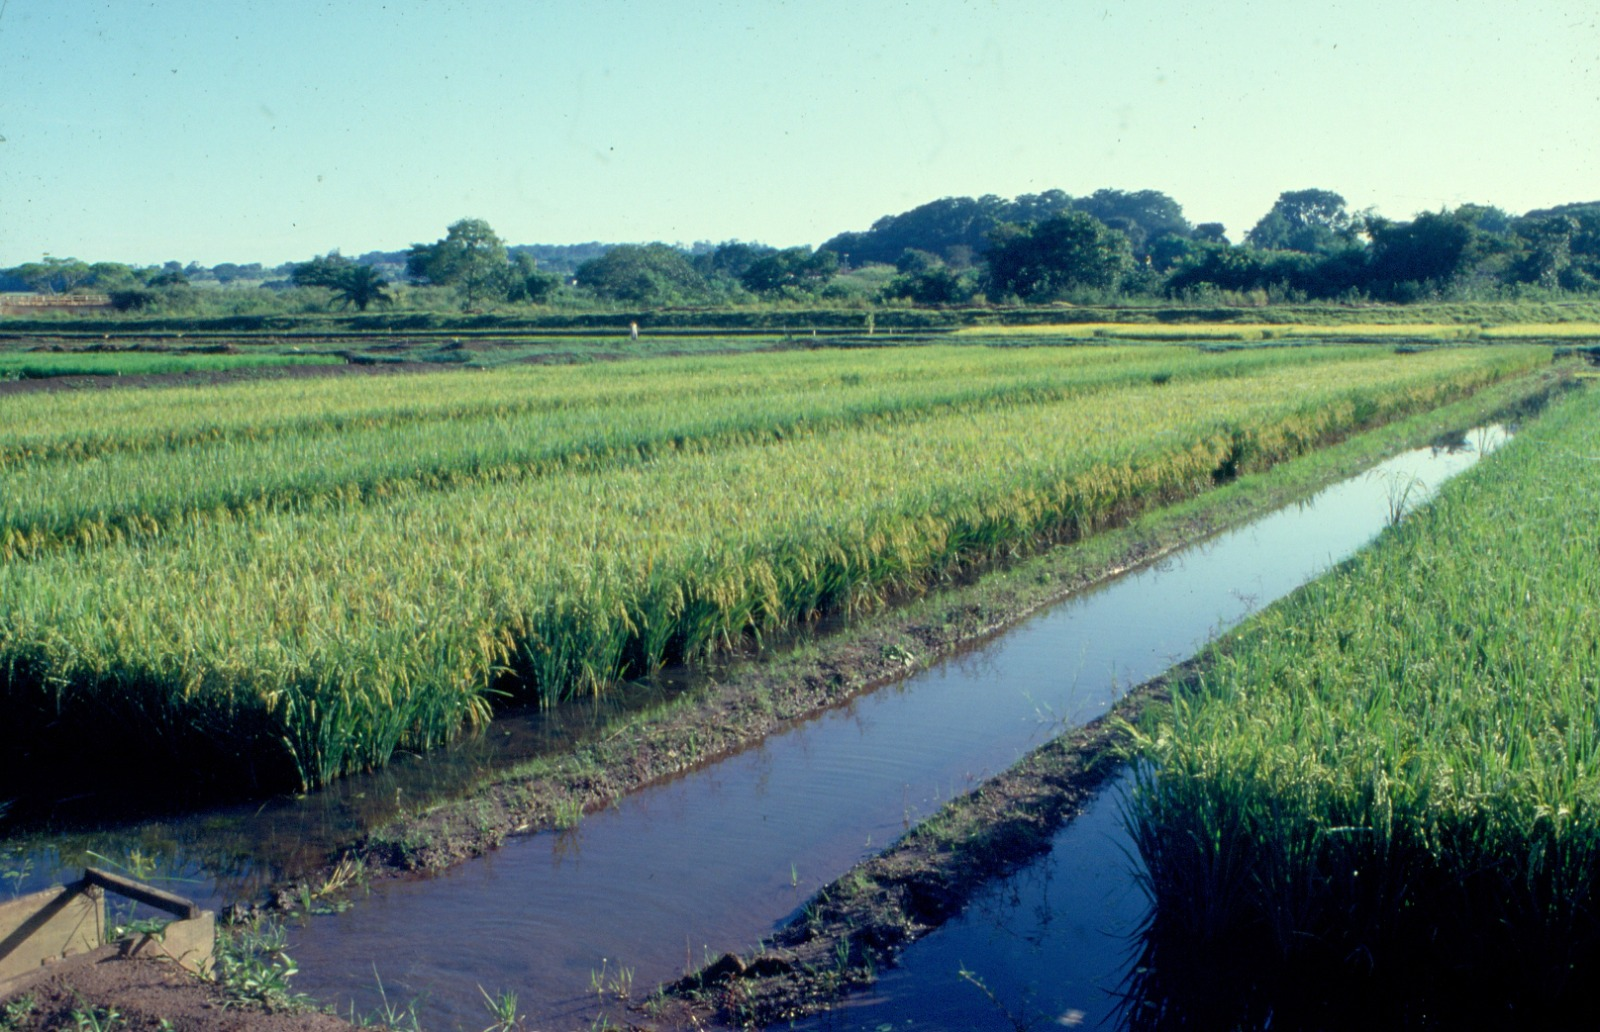
\includegraphics[width=\linewidth]{../images/cultivo do arroz.png}\\[0.1cm]
    {\tiny\textit{Figura 6.1: Cultivo de arroz com lâmina de irrigação.}}
  \end{minipage}
  \hfill
  \begin{minipage}{0.48\textwidth}
    \centering
    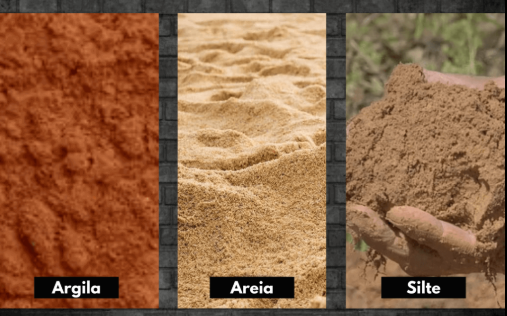
\includegraphics[width=\linewidth]{../images/textura de solo.png}\\[0.1cm]
    {\tiny\textit{Figura 6.2: Classes de textura do solo.}}
  \end{minipage}
\end{center}

\small
A textura do solo é uma das propriedades físicas mais importantes para o planejamento e manejo de bacias de irrigação, especialmente em sistemas de arroz irrigado por lâmina d’água (arroz de várzea). Ela é definida pela proporção relativa das frações de argila, areia e silte presentes no solo e determina características essenciais como capacidade de retenção de água, velocidade de infiltração, porosidade e disponibilidade de nutrientes para as plantas.

No cultivo do arroz de várzea, a manutenção de uma lâmina de água constante sobre o solo é fundamental para o desenvolvimento da cultura. Para isso, solos de textura argilosa ou franco-argilosa são considerados ideais, pois apresentam alta retenção hídrica e baixa taxa de infiltração, o que reduz perdas de água por percolação profunda e facilita o controle da irrigação.

Além disso, solos com maior teor de argila possuem elevada microporosidade e maior capacidade de troca catiônica (CTC), o que favorece a retenção de nutrientes e a eficiência do uso da água pela planta. No entanto, esses solos também exigem manejo cuidadoso para evitar compactação excessiva e garantir adequada aeração e desenvolvimento radicular.

Compreender a textura do solo e suas implicações hidrológicas é, portanto, etapa indispensável para o dimensionamento correto de bacias de irrigação, a definição de lâminas de água adequadas e a adoção de práticas de manejo que maximizem a produtividade do arroz irrigado de forma sustentável.

\vspace{0.2cm}
\scriptsize
\textbf{Referência Bibliográfica:}\\
MASCARENHAS, I. S.; GONÇALVES, G. de M. O.; CAETANO, P. H. P.; SANTOS, A. B. dos; MADARI, B. E.; CORRECHEL, V.; SILVA, M. A. S. da. \textit{Características físicas de solos de várzea e produtividade do arroz irrigado por inundação}. Brasília, DF: Empresa Brasileira de Pesquisa Agropecuária (Embrapa), 2016. Resumo em anais e proceedings. Acesso em: 31 jul. 2026.

\vspace{1cm}
\noindent

Do ponto de vista quantitativo, a determinação da textura do solo deve obedecer ao princípio de conservação de massa das frações granulométricas. Assim, a soma das porcentagens de argila, areia e silte deve satisfazer a seguinte restrição:

\begin{equation}
\text{Argila (\%)} + \text{Areia (\%)} + \text{Silte (\%)} = 100\%
\label{eq:balanco_granulometrico}
\end{equation}

Essa condição é fundamental para a correta classificação textural do solo por meio do triângulo textural (USDA ou sistema brasileiro), garantindo que as proporções estejam coerentes e que a classe textural identificada represente adequadamente as propriedades físico-hídricas do solo . Com base nas implicações agronômicas da textura para o arroz irrigado, pode-se definir um \textbf{Índice de Aptidão (Fitness)} do solo para essa cultura. Esse índice empírico pondera positivamente as frações de argila e silte (benéficas para retenção hídrica) e negativamente a fração de areia (associada à maior infiltração e menor retenção):

\begin{equation}
\text{Fitness} = \left(1.5 \times \text{Argila}\right) + \left(0.8 \times \text{Silte}\right) - \left(0.5 \times \text{Areia}\right)
\label{eq:fitness}
\end{equation}

\noindent
em que \textit{Argila}, \textit{Silte} e \textit{Areia} são expressos em porcentagem (\%) e satisfazem a Equação~\ref{eq:balanco_granulometrico}.

Quanto maior o valor de \textit{Fitness}, maior a aptidão textural do solo para o cultivo de arroz irrigado por inundação. Solos argilosos e franco-argilosos, típicos de várzeas, tendem a apresentar valores elevados desse índice, refletindo sua adequação para a manutenção da lâmina d'água e eficiência no uso de nutrientes .

A combinação da restrição granulométrica (Eq.~\ref{eq:balanco_granulometrico}) com o índice de aptidão (Eq.~\ref{eq:fitness}) oferece uma base quantitativa para o planejamento de bacias de irrigação, seleção de áreas para expansão do arroz irrigado e avaliação de estratégias de manejo que maximizem a produtividade de forma sustentável.

\vspace{0.3cm}

\vspace{0.2cm}
\noindent
Considere a seguinte classificação de aptidão para a cultura do arroz irrigado:
\begin{itemize}[leftmargin=1.5em]
  \item $\text{Fitness} \ge 60.0$: Excelente Aptidão (Alta retenção hídrica)
  \item $40.0 \le \text{Fitness} < 60.0$: Aptidão Moderada (Requer maior manejo de irrigação)
  \item $\text{Fitness} < 40.0$: Inadequado (Solo excessivamente permeável/arenoso)
\end{itemize}

\vspace{0.3cm}
% Diagrama UML TikZ para Solo
\begin{center}
\begin{tikzpicture}[
  font=\sffamily\small,
  umlclass/.style={draw=maincolor, fill=blue!5, line width=1pt, rounded corners=2pt, inner sep=6pt, text width=11.5cm}
]
\node[umlclass] (solo) {
  \centering \textbf{Solo}\\[2pt]
  \hrulefill\\
  + identificacao: String\\
  + argila: Double\\
  + areia: Double\\
  + silte: Double\\
  \hrulefill\\
  + constructor(identificacao: String, argila: Double, areia: Double, silte: Double)\\
  + validarTextura(): Boolean\\
  + calcularFitness(): Double\\
  + obterClassificacao(): String\\
  + compararAptidao(outroSolo: Solo): Solo\\
  + exibirRelatorio(): Unit
};
\end{tikzpicture}
\end{center}

\vspace{0.2cm}
\noindent
\textbf{Especificações de Implementação em Kotlin:}
\begin{enumerate}[label=\alph*), leftmargin=1.5em]
  \item Implemente o construtor da classe `Solo`. No bloco `init`, valide se $\text{argila} + \text{areia} + \text{silte} = 100.0$ (tolere pequenas diferenças de arredondamento de $\pm 0.1$). Caso inválido, exiba um aviso.
  \item Implemente o método `calcularFitness(): Double` com a fórmula fornecida.
  \item Implemente o método `obterClassificacao(): String` que retorna o texto da aptidão.
  \item Método de Comparação: Implemente `compararAptidao(outroSolo: Solo): Solo`, que compara o *fitness* do solo atual (\texttt{this}) com o de `outroSolo` recebido como parâmetro e retorna o objeto `Solo` que possui a melhor aptidão (maior fitness) para o cultivo de arroz irrigado.
  \item Na função `main()`, instancie dois solos (ex: *Lote A: 50\% Argila, 20\% Areia, 30\% Silte* e *Lote B: 15\% Argila, 70\% Areia, 15\% Silte*), exiba os relatórios de cada um e utilize o método `compararAptidao` para indicar qual solo é mais recomendado.
\end{enumerate}

\vspace{0.2cm}
\begin{block}{Exemplo de Entrada e Saída Esperada (Console)}
\textbf{Objetos Instanciados:}\\
\texttt{soloA = Solo("Lote A", argila=50.0, areia=20.0, silte=30.0)}\\
\texttt{soloB = Solo("Lote B", argila=15.0, areia=70.0, silte=15.0)}\\
\textbf{Saída de Console:}
\begin{verbatim}
--- Relatório de Solo: Lote A ---
Composição: 50.0% Argila, 20.0% Areia, 30.0% Silte
Índice de Fitness: 89.0
Classificação: Excelente Aptidão (Alta retenção hídrica)

--- Relatório de Solo: Lote B ---
Composição: 15.0% Argila, 70.0% Areia, 15.0% Silte
Índice de Fitness: -0.5
Classificação: Inadequado (Solo excessivamente permeável/arenoso)

=======================================================
Resultado da Comparação de Aptidão:
O solo recomendado para cultivo de arroz irrigado é: Lote A (Fitness: 89.0)
=======================================================
\end{verbatim}
\end{block}

% =========================
\end{document}
% =========================
